\chapter{Empirical Risk}
As we already stated, ML aims at learning a \textbf{hypothesis} $h$: a function that reads the \textbf{features} $x$ of a data point and returns a prediction of its \textbf{label} $y$. A \textbf{data point} $(x,y)$ is any object we are interested in. 

We want $h(x)$ to be close to $y$ not only for the data points we already have, but for \textbf{any data point we might encounter} in the future.\\

\begin{center}
    \textit{To reason about data we have not seen yet, we need a probabilistic model. Data points are interpreted as realizations of \textbf{random variables (RVs)}. A RV is a quantity whose value depends on the outcome of a random experiment, and a realization is the specific value we observe. These RVs are assumed to be \textbf{i.i.d.} (independent and identically distributed): data points do not influence each other (independent), and all of them are generated by the same \textbf{probability distribution} $p(x,y)$ (identically distributed). }
\end{center}

To measure how wrong a prediction is, we use a \textbf{loss function}, which assigns a non-negative number to each data point: the larger the loss, the worse the prediction $h(x)$ compared to the true label $y$. However, the loss on a single data point says little about $h$ in general. What we really care about is the \textbf{expected loss}, also called \textbf{expected risk}: the average loss of $h$ over all possible data points, where each point is weighted by how likely it is according to $p(x,y)$. A hypothesis with \textcolor{red}{small expected risk makes good predictions on future data}.\\

The problem is that computing the expected risk requires knowing $p(x,y)$, which in practice is never available. What we do have is a finite set of labelled data points, the \textbf{training set}. The idea is therefore to approximate the expected risk with the \textbf{empirical risk}, defined as the \textbf{average loss on the data points of the training set}. Since the training points are i.i.d. samples of $p(x,y)$, the empirical risk is a reasonable estimate of the expected risk. \textcolor{red}{This estimate becomes more accurate as the number of training points grows}.\\

\begin{figure}[h]
    \centering
    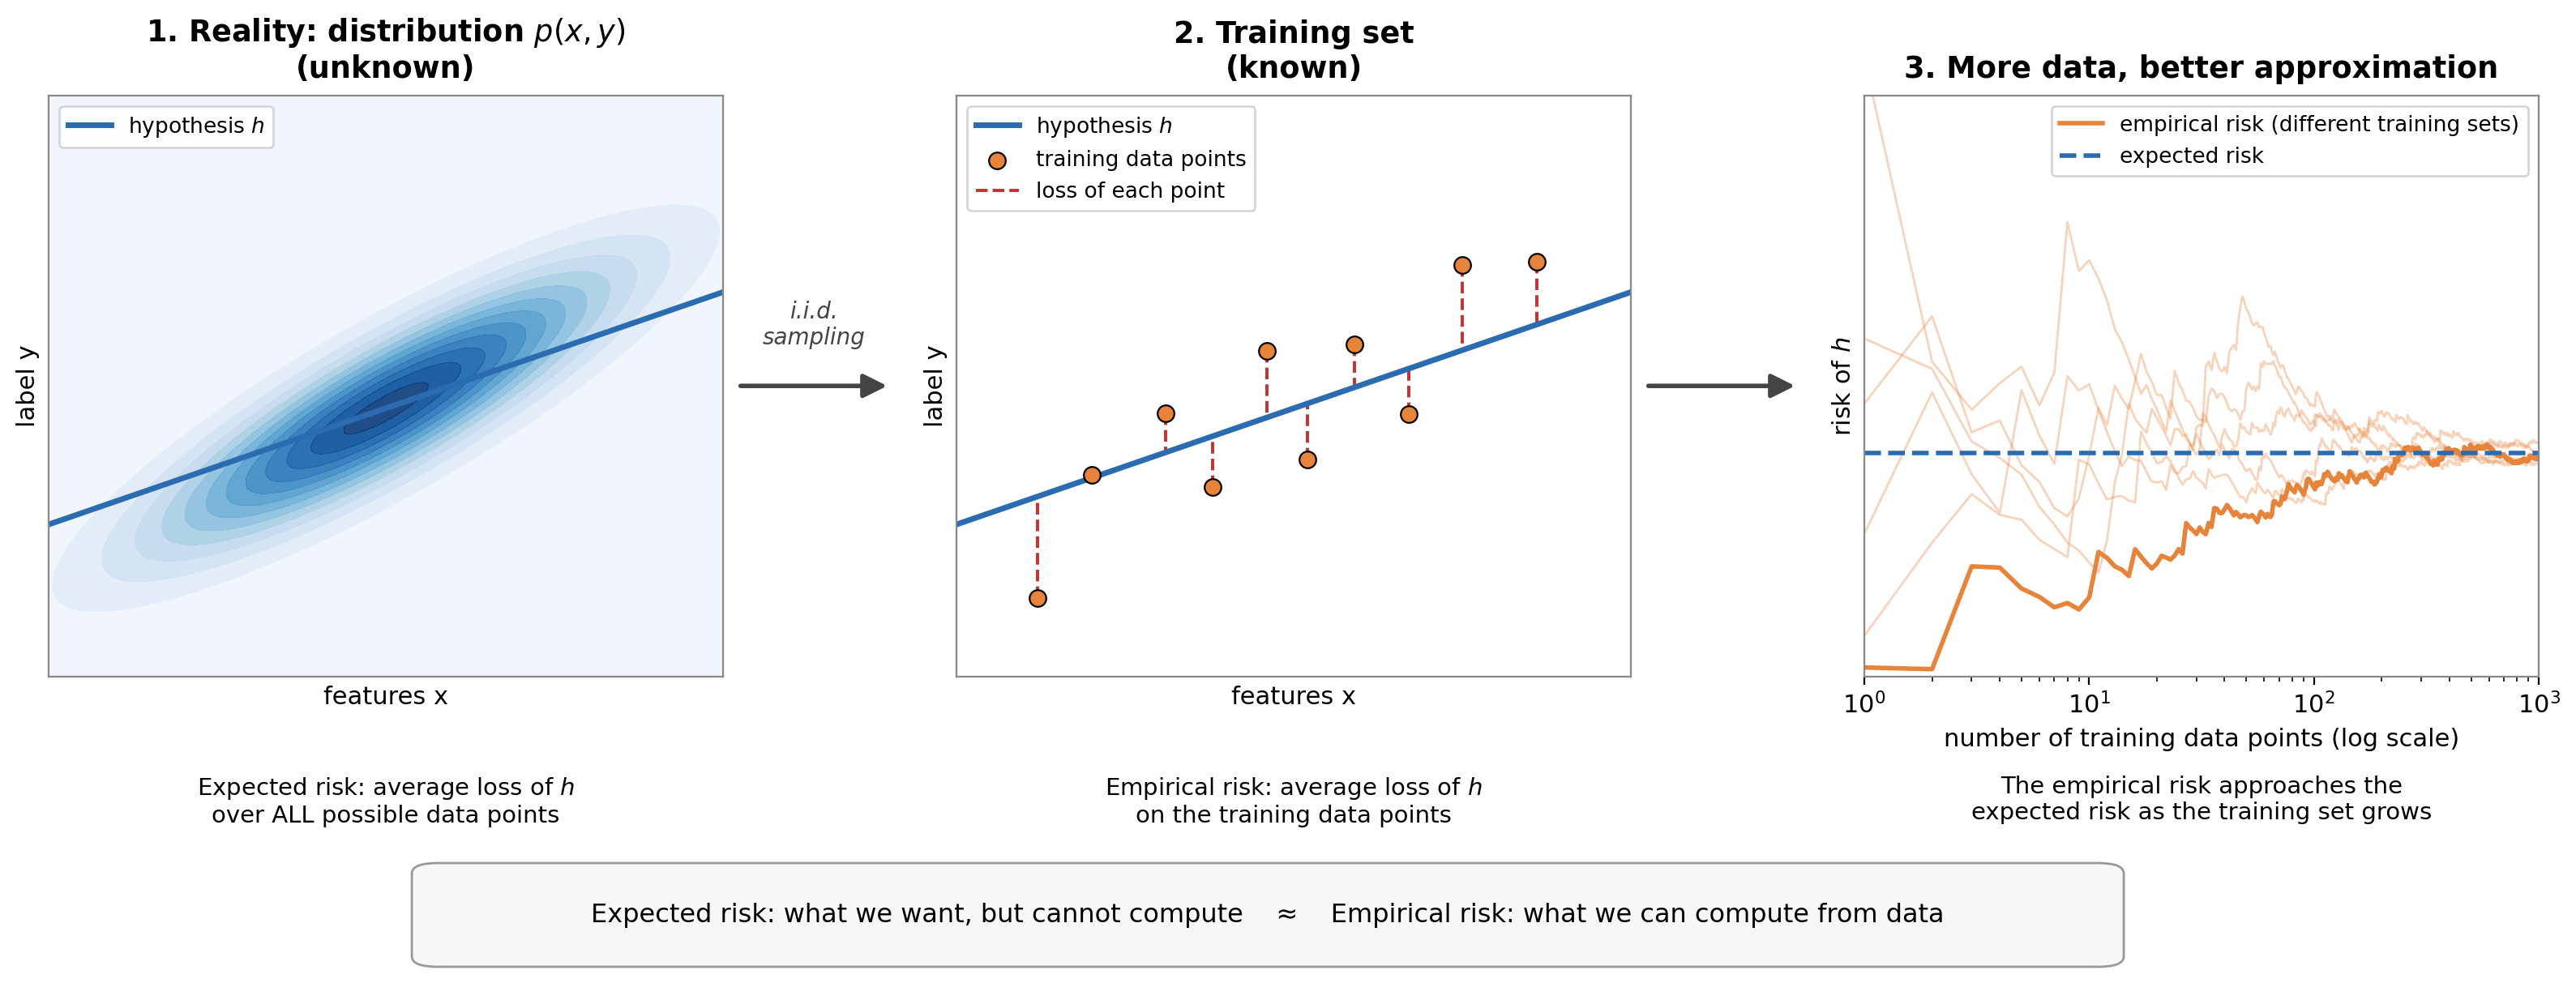
\includegraphics[width=1\textwidth]{images/chapter_6/ch_empirical_risk.png}
    \caption{From the unknown distribution $p(x,y)$ to the training set: the empirical risk approximates the expected risk, and the approximation improves as the training set grows.}
\end{figure}

In short, the expected risk is what we would like to minimize but cannot compute, while the empirical risk is what we can compute and use in its place.

\section{Empirical Risk Minimization}
\textbf{Empirical Risk Minimization} (ERM) turns the idea of the previous section into a learning principle. Among all hypotheses of the \textbf{hypothesis space} (the model), we choose the one with the \textbf{smallest empirical risk}, i.e. the one that makes the smallest average loss when predicting the \textbf{labels} of the training data points from their \textbf{features}.

When the hypotheses are described by a parameter vector (for instance the weights of a linear map), choosing the best hypothesis means choosing the best parameter vector. Learning therefore becomes an \textbf{optimization problem}: find the parameters that minimize the empirical risk.

It is important to keep in mind that ERM only looks at the training data. It works well as long as the empirical risk is a good approximation of the expected risk; when the two differ, the hypothesis that is best on the training set may not be the best on new data.

\begin{figure}[h]
    \centering
    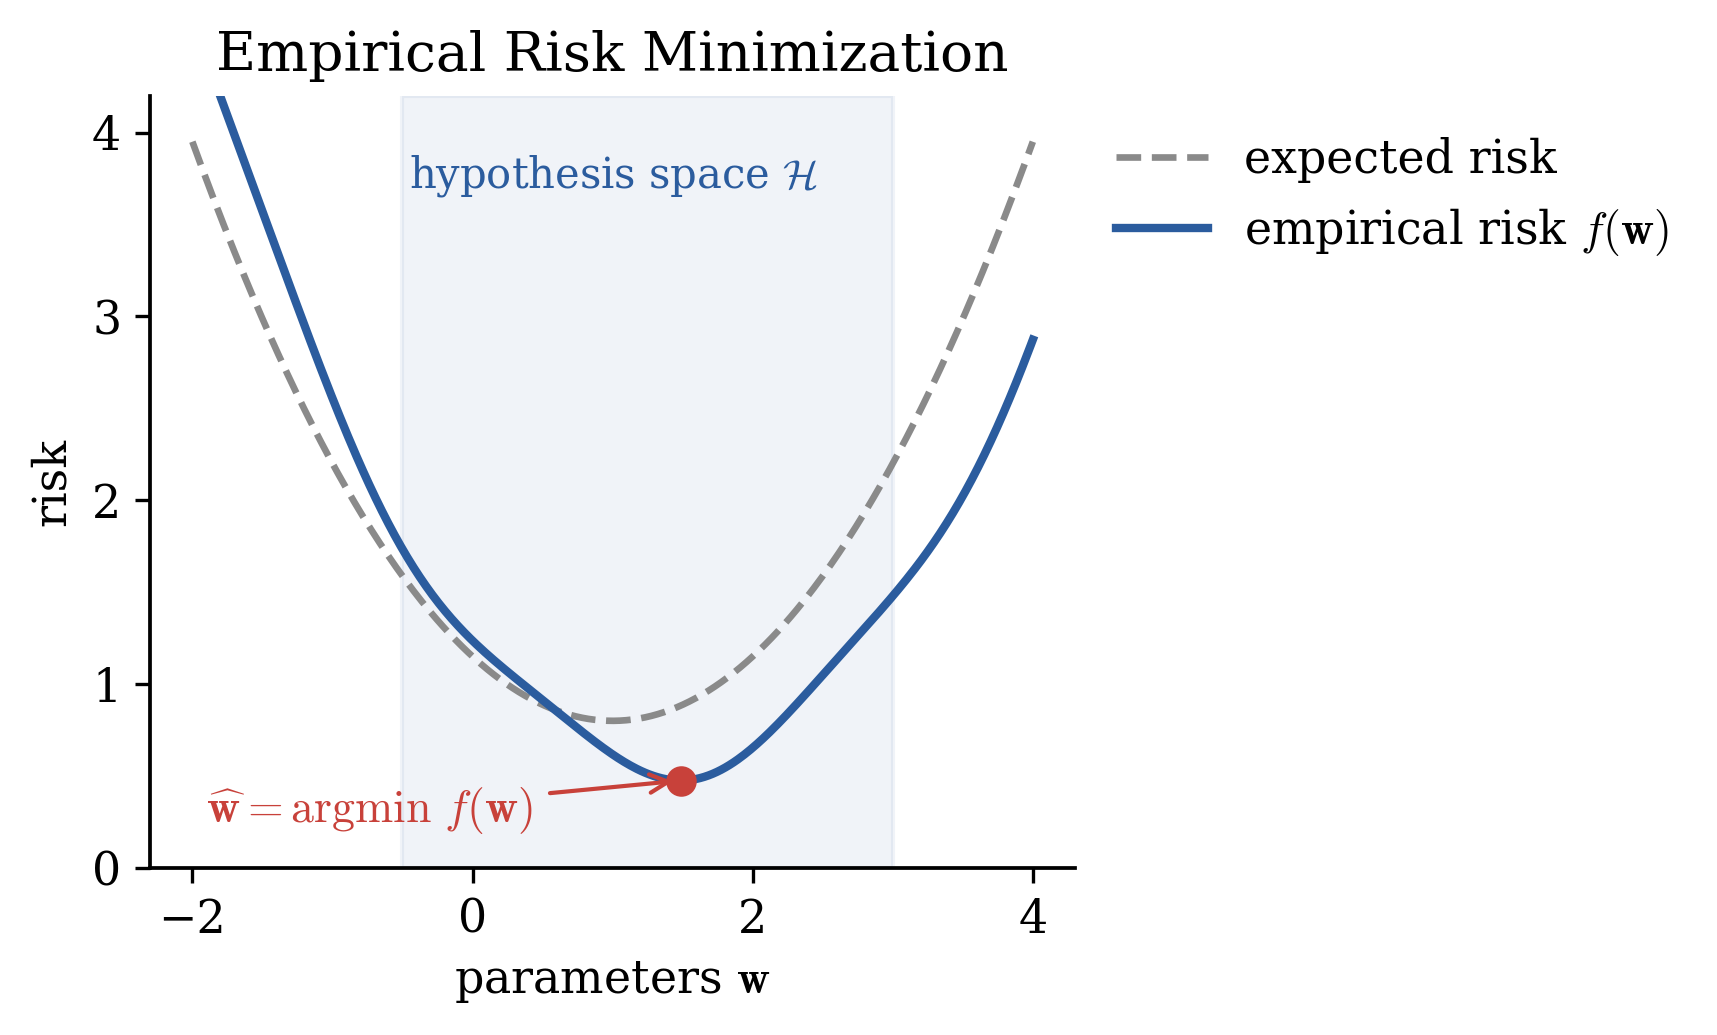
\includegraphics[width=0.8\textwidth]{images/chapter_6/sec_erm.png}
    \caption{Empirical risk vs expected risk and optimal parameter vector}
\end{figure}

\section{ERM for regression}
ERM can be applied to different kinds of problems, which mainly differ in the type of label:

\begin{itemize}
    \item \textbf{Regression}: the label is a \textbf{number} that can take continuous values (e.g. a price or a temperature). The loss measures the \textbf{distance} between the predicted number and the true one.
    \item \textbf{Classification}: the label is a \textbf{category}, chosen among two classes (binary) or more (multi-class). Since we cannot measure a ``distance'' between categories, the loss is based on how \textbf{confident} the prediction is and whether it is correct.
\end{itemize}

\begin{figure}[h]
    \centering
    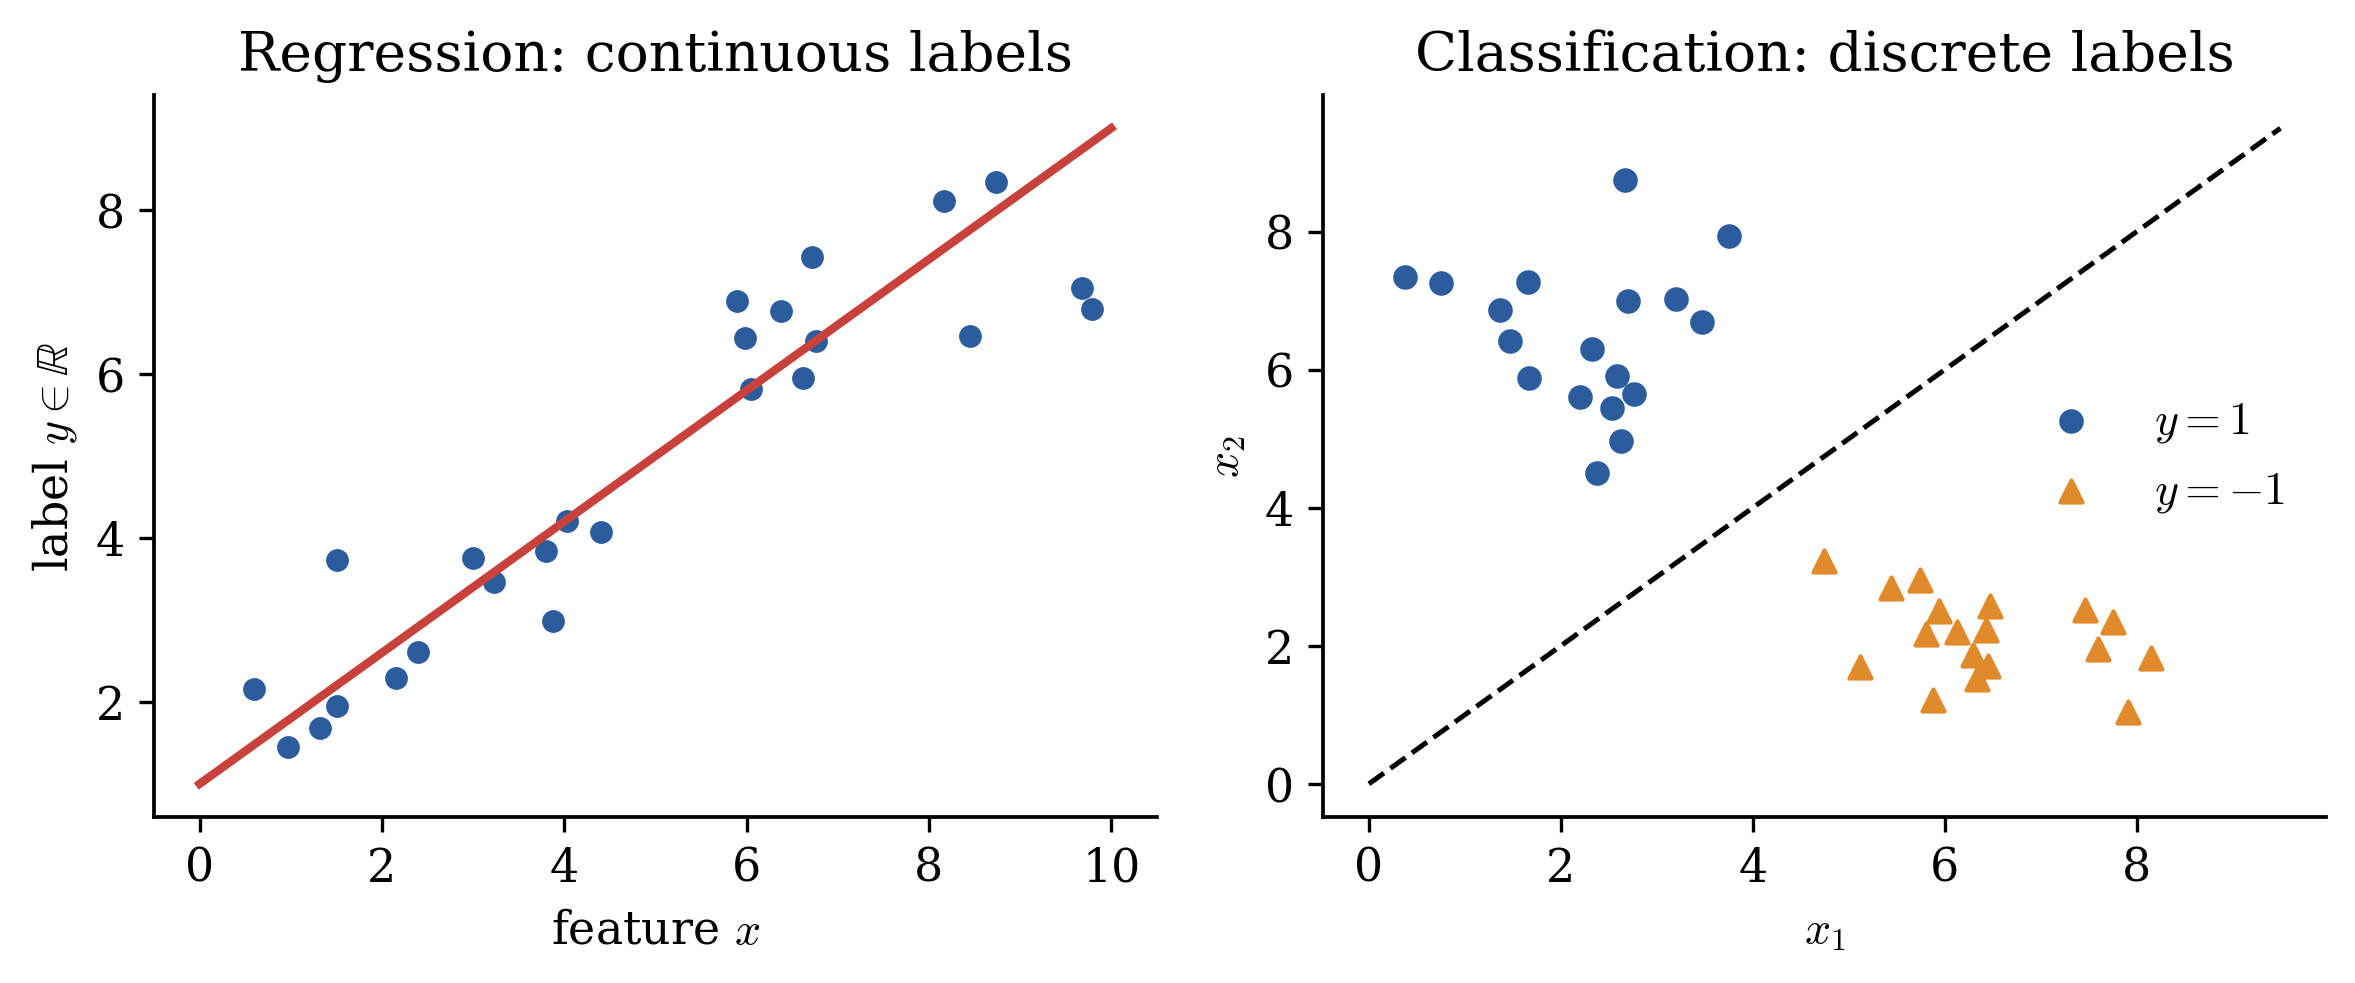
\includegraphics[width=0.9\textwidth]{images/chapter_6/sec_erm_regression.png}
    \caption{Regression vs Classification}
\end{figure}

\subsection{Linear Regression}
Linear regression is ERM with the following three choices:

\begin{itemize}
    \item \textbf{Data}: each data point has a \textbf{numeric feature vector} and a \textbf{numeric label}.
    \item \textbf{Model}: \textbf{linear hypothesis maps}, i.e. the prediction is a weighted sum of the features.
    \item \textbf{Loss}: \textbf{squared error loss}.
\end{itemize}

A straight line is often too simple to describe the data. \textbf{Polynomial Regression} solves this by first transforming the features into their powers ($x, x^2, \dots, x^n$) and then applying ordinary linear regression to these new features. The resulting hypothesis is a polynomial of degree $n$ in the original feature, but it is still \emph{linear in the parameters}. In other words, the model becomes larger and more flexible, while the method stays exactly the same.

\begin{figure}[h]
    \centering
    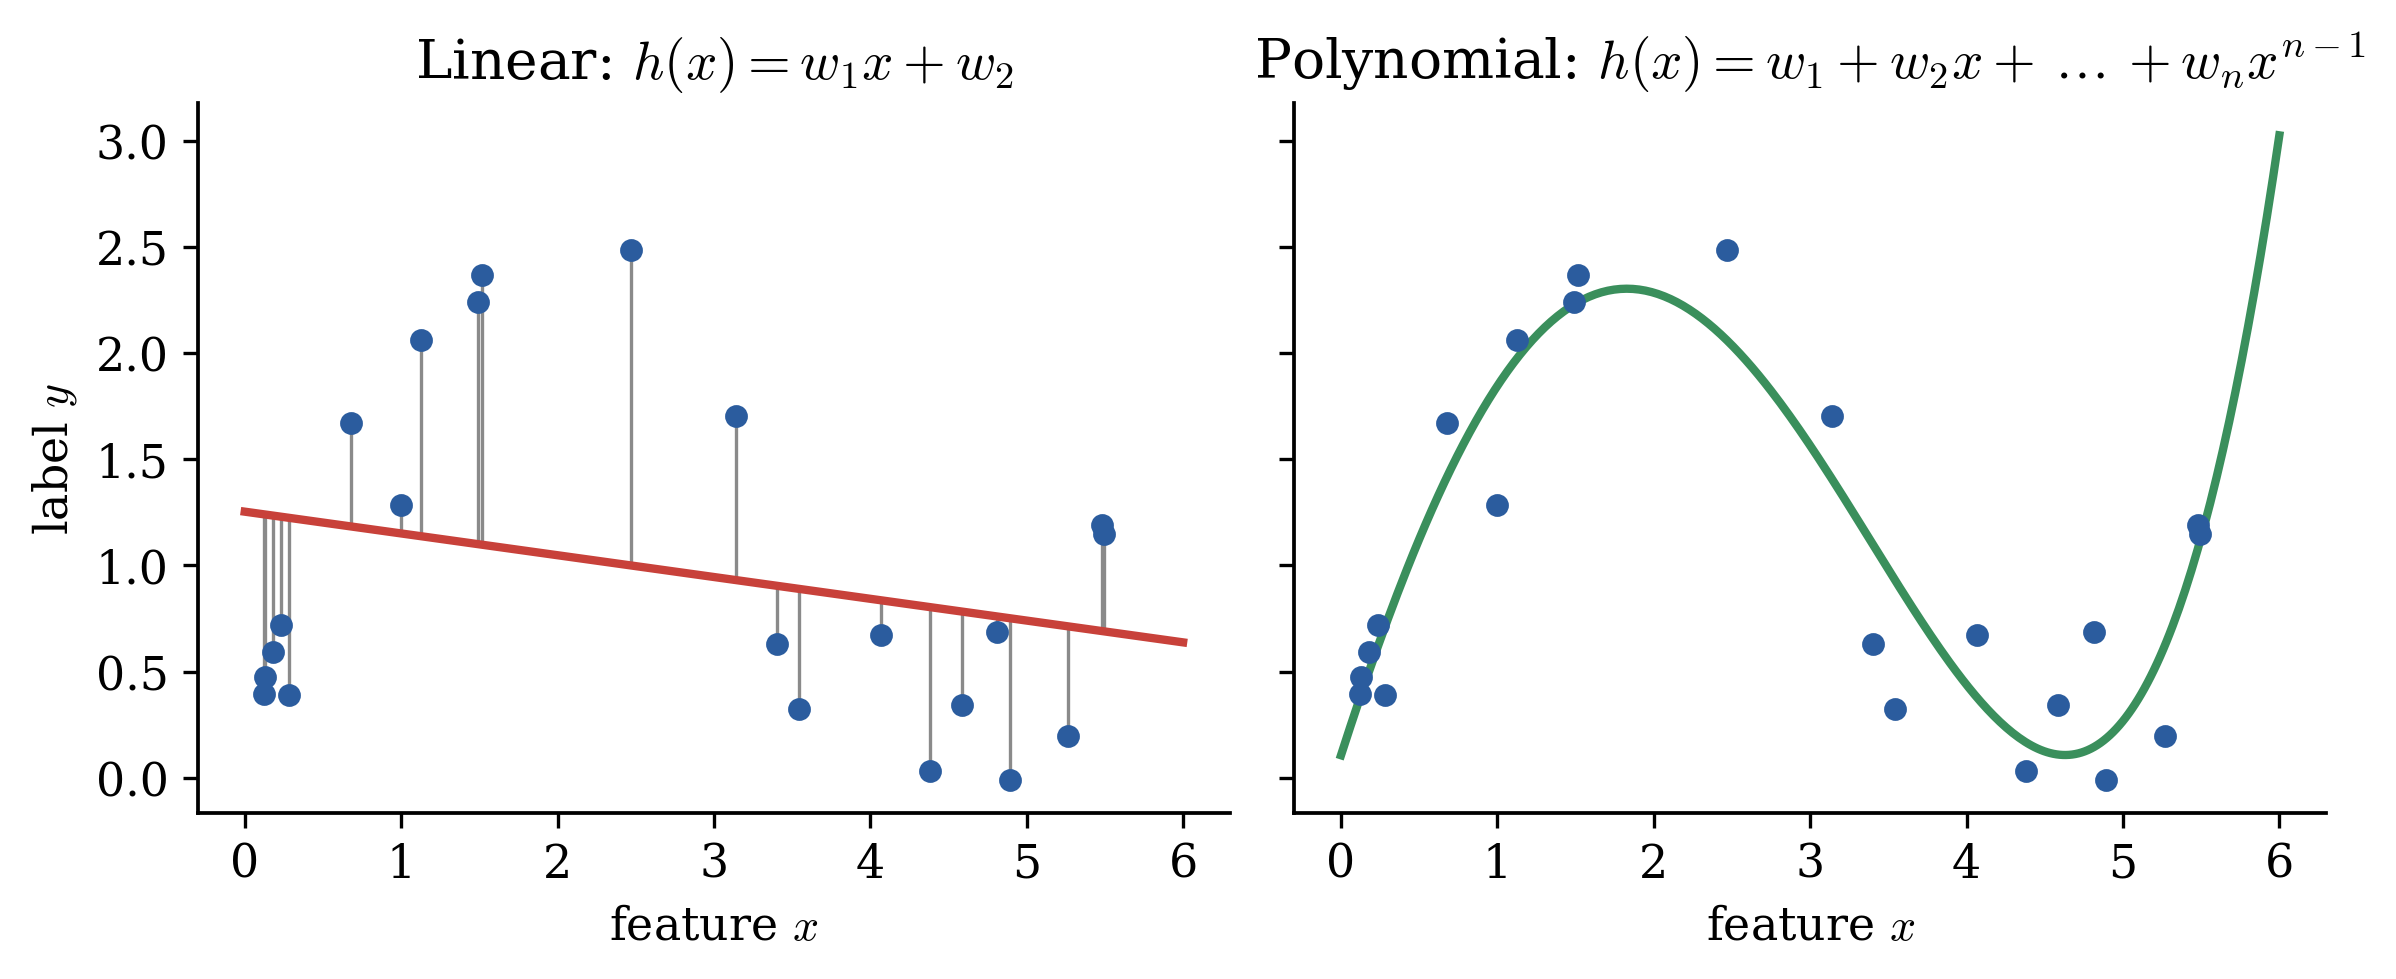
\includegraphics[width=0.9\textwidth]{images/chapter_6/sub_linear_regression.png}
    \caption{Linear Regression vs Polynomial Regression}
\end{figure}

\subsection{Loss Functions for regression}
The loss function decides \textbf{how much each error counts}. All regression losses are zero when the prediction is exact and grow as the prediction moves away from the true label; what changes is \textbf{how fast they grow}, and therefore how they treat large errors such as those caused by \textbf{outliers}. We consider three of them:

\begin{itemize}
    \item Squared Error Loss
    \item Absolute Error Loss
    \item Huber Loss
\end{itemize}

\begin{figure}[h]
    \centering
    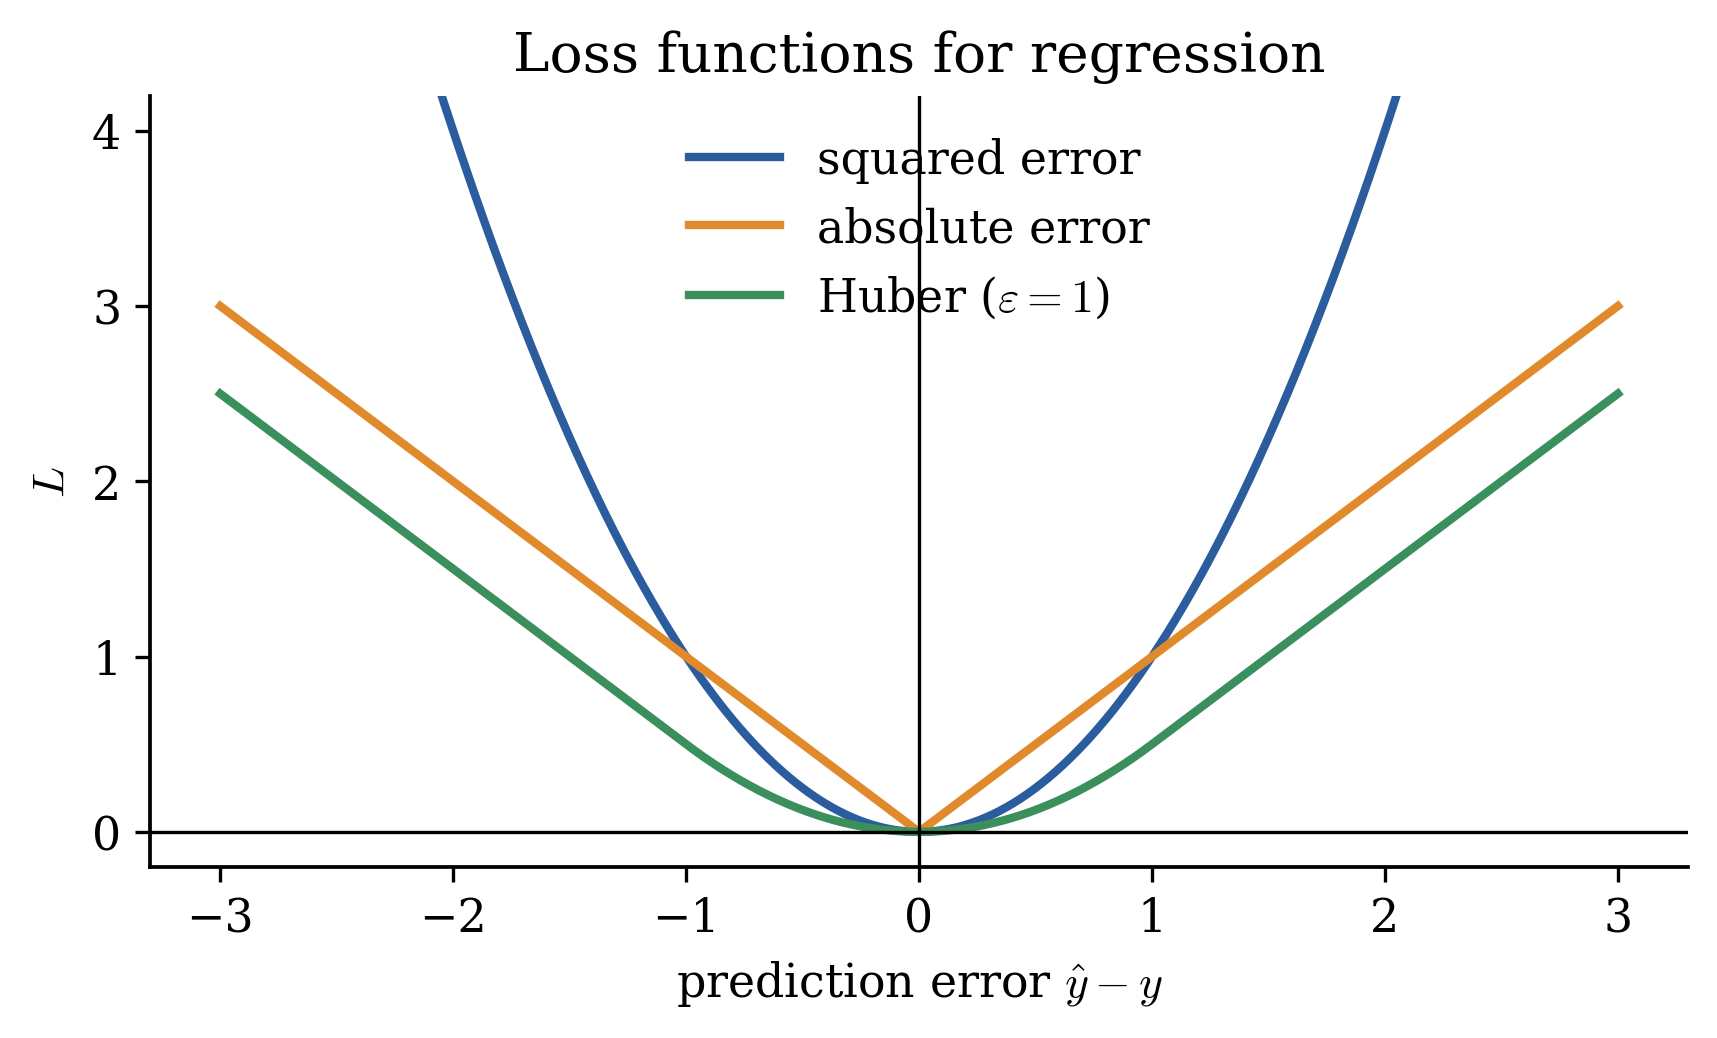
\includegraphics[width=0.65\textwidth]{images/chapter_6/sub_losses_regression.png}
    \caption{Loss functions for regression}
\end{figure}

\subsection{Squared Error Loss}
The squared error loss is defined as:
\[
L := (\widehat{y} - y)^2
\]

\begin{figure}[h]
    \centering
    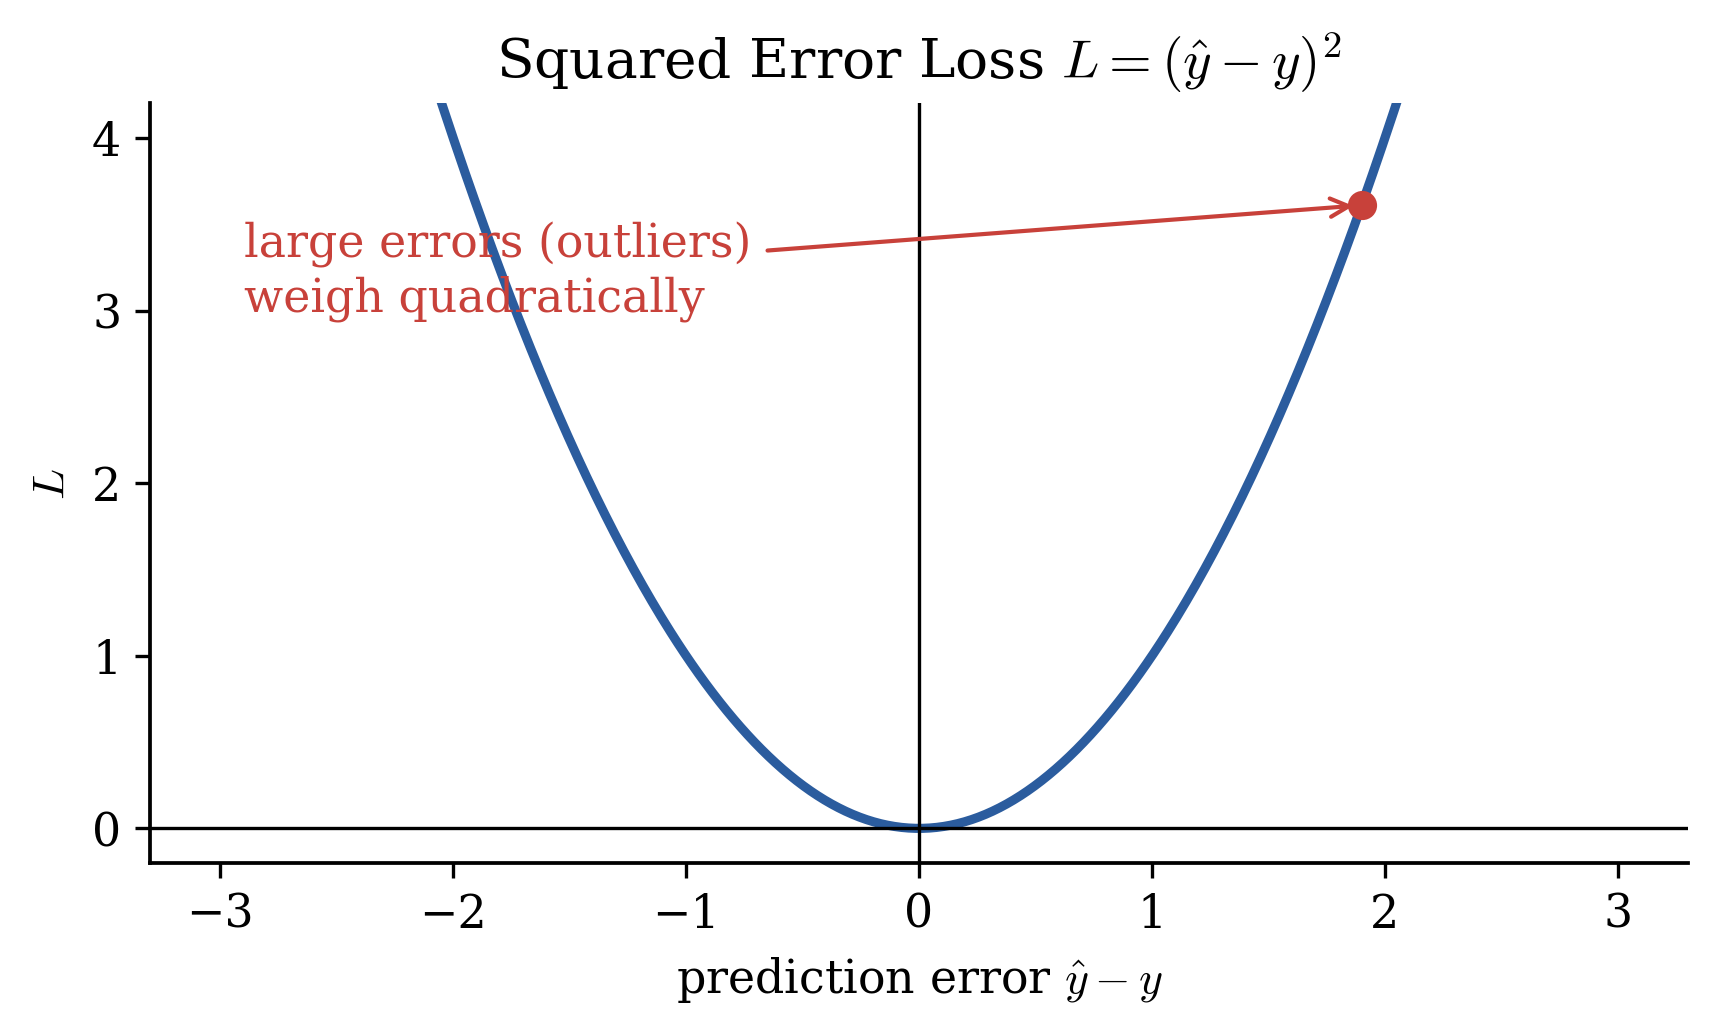
\includegraphics[width=0.65\textwidth]{images/chapter_6/sub_squared_loss.png}
    \caption{Squared Error Loss}
\end{figure}

Squaring makes large errors weigh much more than small ones: an error of 10 costs 100, while an error of 1 costs only 1. As a consequence, a single outlier can dominate the empirical risk and \textbf{pull the predictor towards itself}. On the other hand, the squared error is convex and differentiable, so it is easy to minimize. It is a good choice when the data contain \textbf{no outliers}.

\subsection{Absolute Error Loss}

The absolute error loss is defined as:
\[
L := |\widehat{y} - y|
\]

\begin{figure}[h]
    \centering
    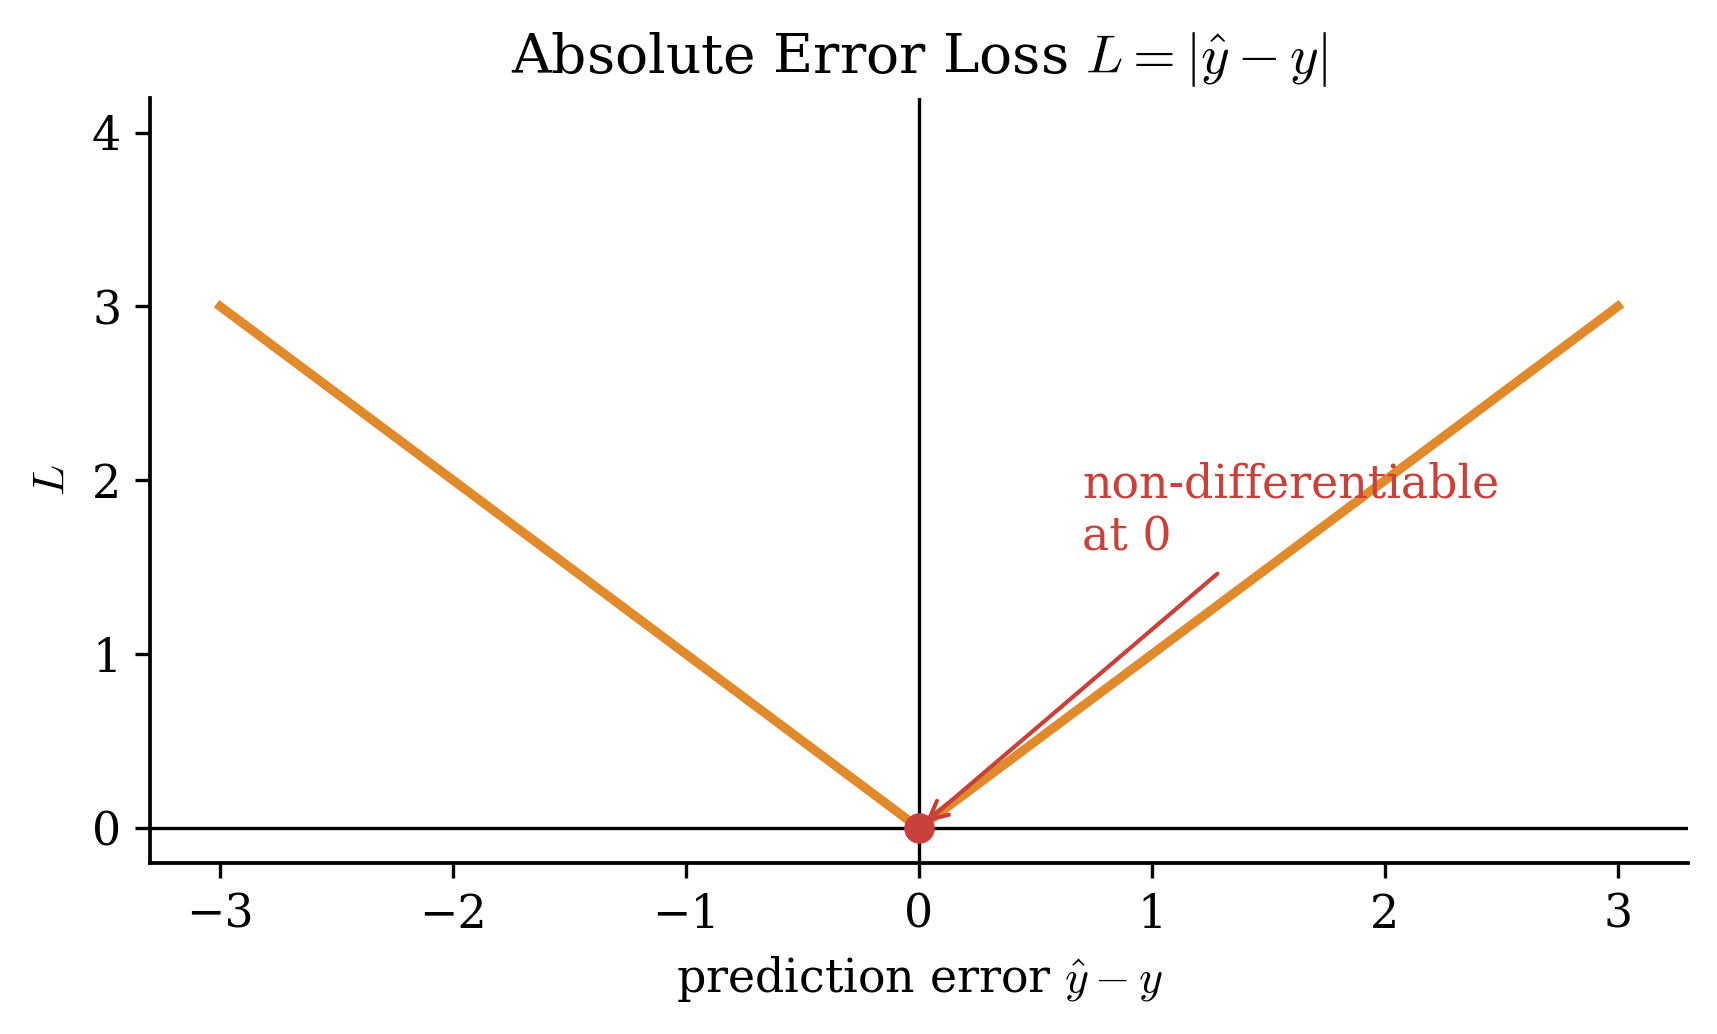
\includegraphics[width=0.65\textwidth]{images/chapter_6/sub_absolute_loss.png}
    \caption{Absolute Error Loss}
\end{figure}

Here the loss grows only \textbf{linearly} with the error, so an outlier counts in proportion to its distance and cannot dominate the others: the absolute error is \textbf{robust to outliers}. Its drawback is the corner at zero error, where the function is \textbf{not differentiable}. At that point the gradient is not defined, so gradient-based methods do not know in which direction to move.

\subsection{Huber Loss}
The Huber loss is defined as:
\[
L\big((\mathbf{x},y),h\big) =
\begin{cases}
(1/2)(y - h(\mathbf{x}))^2 & \text{for } |y - h(\mathbf{x})| \leq \varepsilon \\
\varepsilon(|y - h(\mathbf{x})| - \varepsilon/2) & \text{else.}
\end{cases}
\]

\begin{figure}[h]
    \centering
    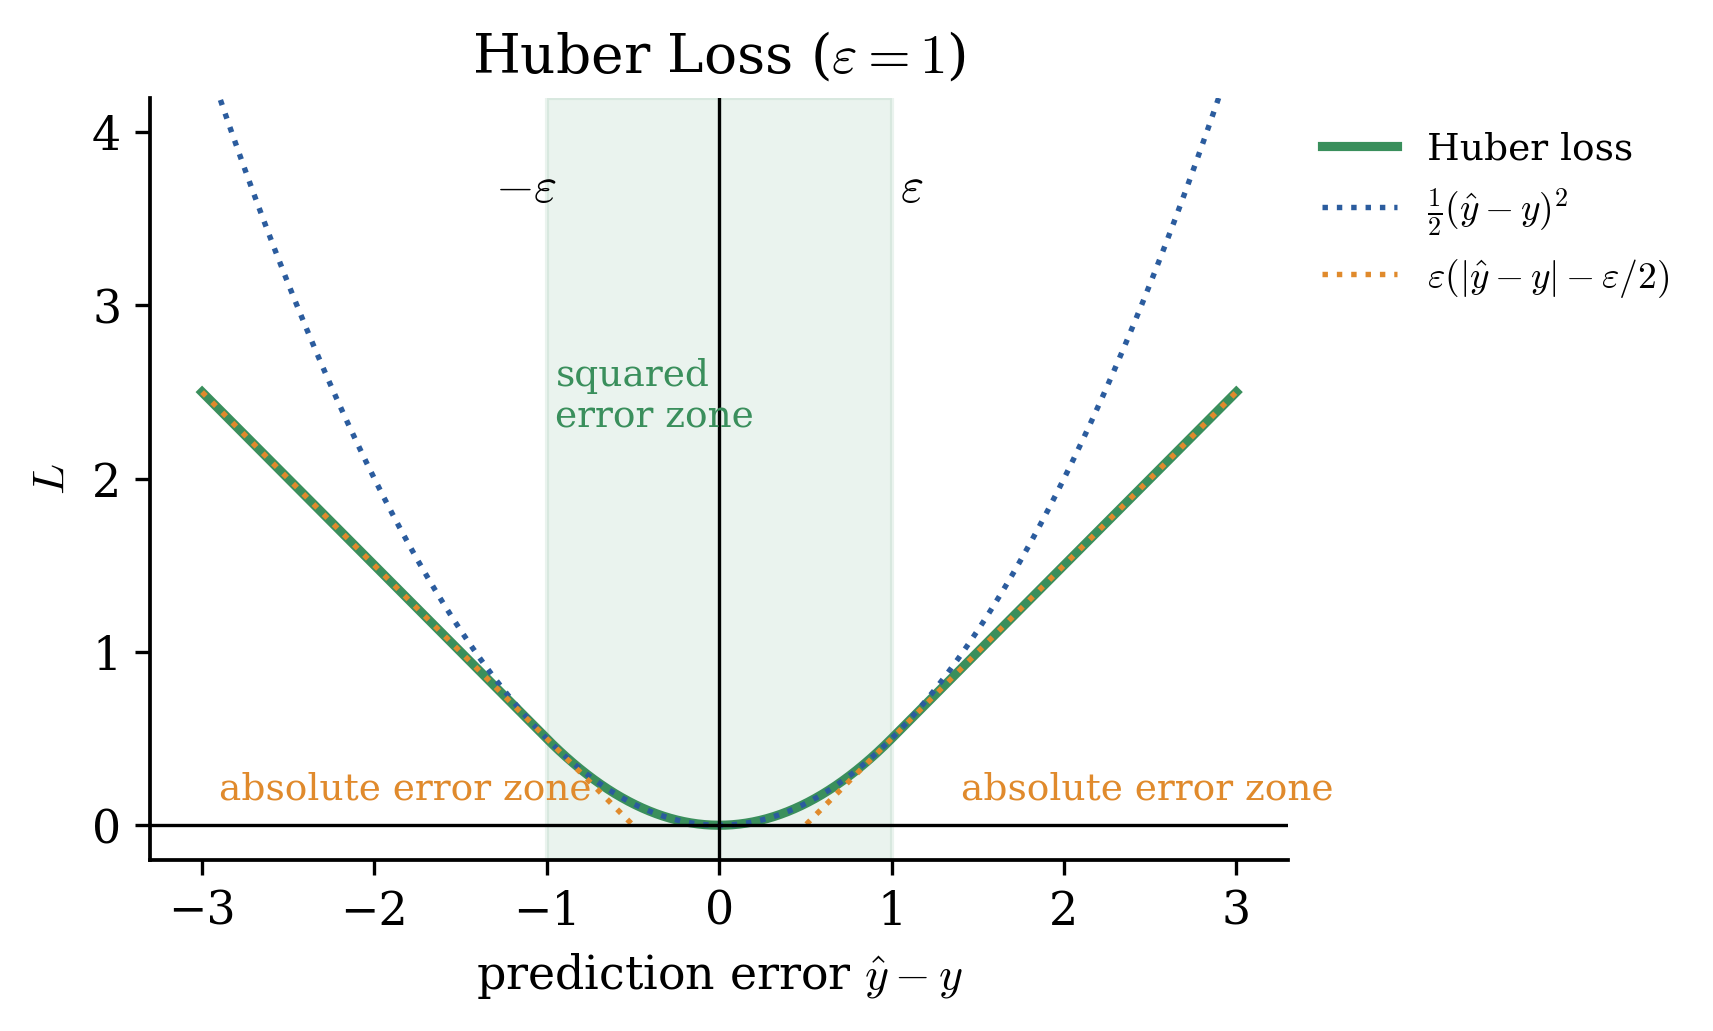
\includegraphics[width=0.8\textwidth]{images/chapter_6/sub_huber_loss.png}
    \caption{Huber Loss}
\end{figure}

The Huber loss combines the strengths of the previous two. For \textbf{small errors} (inside the $\varepsilon$ interval) it behaves like the squared error, so it is smooth and differentiable around zero. For \textbf{large errors} (outside the interval) it behaves like the absolute error, so outliers are tolerated. The constants $1/2$ and $\varepsilon/2$ make the two pieces join smoothly, so the function is differentiable everywhere.

To conclude, here is a comparison of the loss functions for regression:

\begin{center}
    \begin{tabular}{l|c|c|c}
        & \textbf{Robust to outliers} & \textbf{Insensitive to noise} & \textbf{Differentiable} \\ \hline
        Squared Error  & no  & yes & yes \\
        Absolute Error & yes & no  & no  \\
        Huber          & yes & yes & yes \\
    \end{tabular}
\end{center}

\textbf{Insensitive to noise} means that small deviations between the label $y$ and the prediction $h(\mathbf{x})$ have little effect on the loss. Squaring a small number makes it even smaller, which is why the squared error and the Huber loss have this property. All three losses are convex. Loss functions are preferred to be both \textbf{convex} and \textbf{differentiable}, since this makes them easier to minimize.


\section{ERM for Classification}
In classification the label is a \textbf{category}, for instance $y \in \{-1, +1\}$ in binary classification. Between categories there is no meaningful notion of distance, so the losses used for regression cannot be applied directly. The trick is to let the hypothesis still output a \textbf{real number} $h(\mathbf{x})$ and to read it in two parts:

\begin{itemize}
    \item its \textbf{sign} gives the predicted class: positive means $+1$, negative means $-1$;
    \item its \textbf{absolute value} $|h(\mathbf{x})|$ measures the \textbf{confidence} of the prediction: the farther from zero, the more sure the classifier is.
\end{itemize}
A classification loss is then built from this confidence: it should be small when the prediction is correct and confident, and large when it is wrong and confident.

\begin{figure}[h]
    \centering
    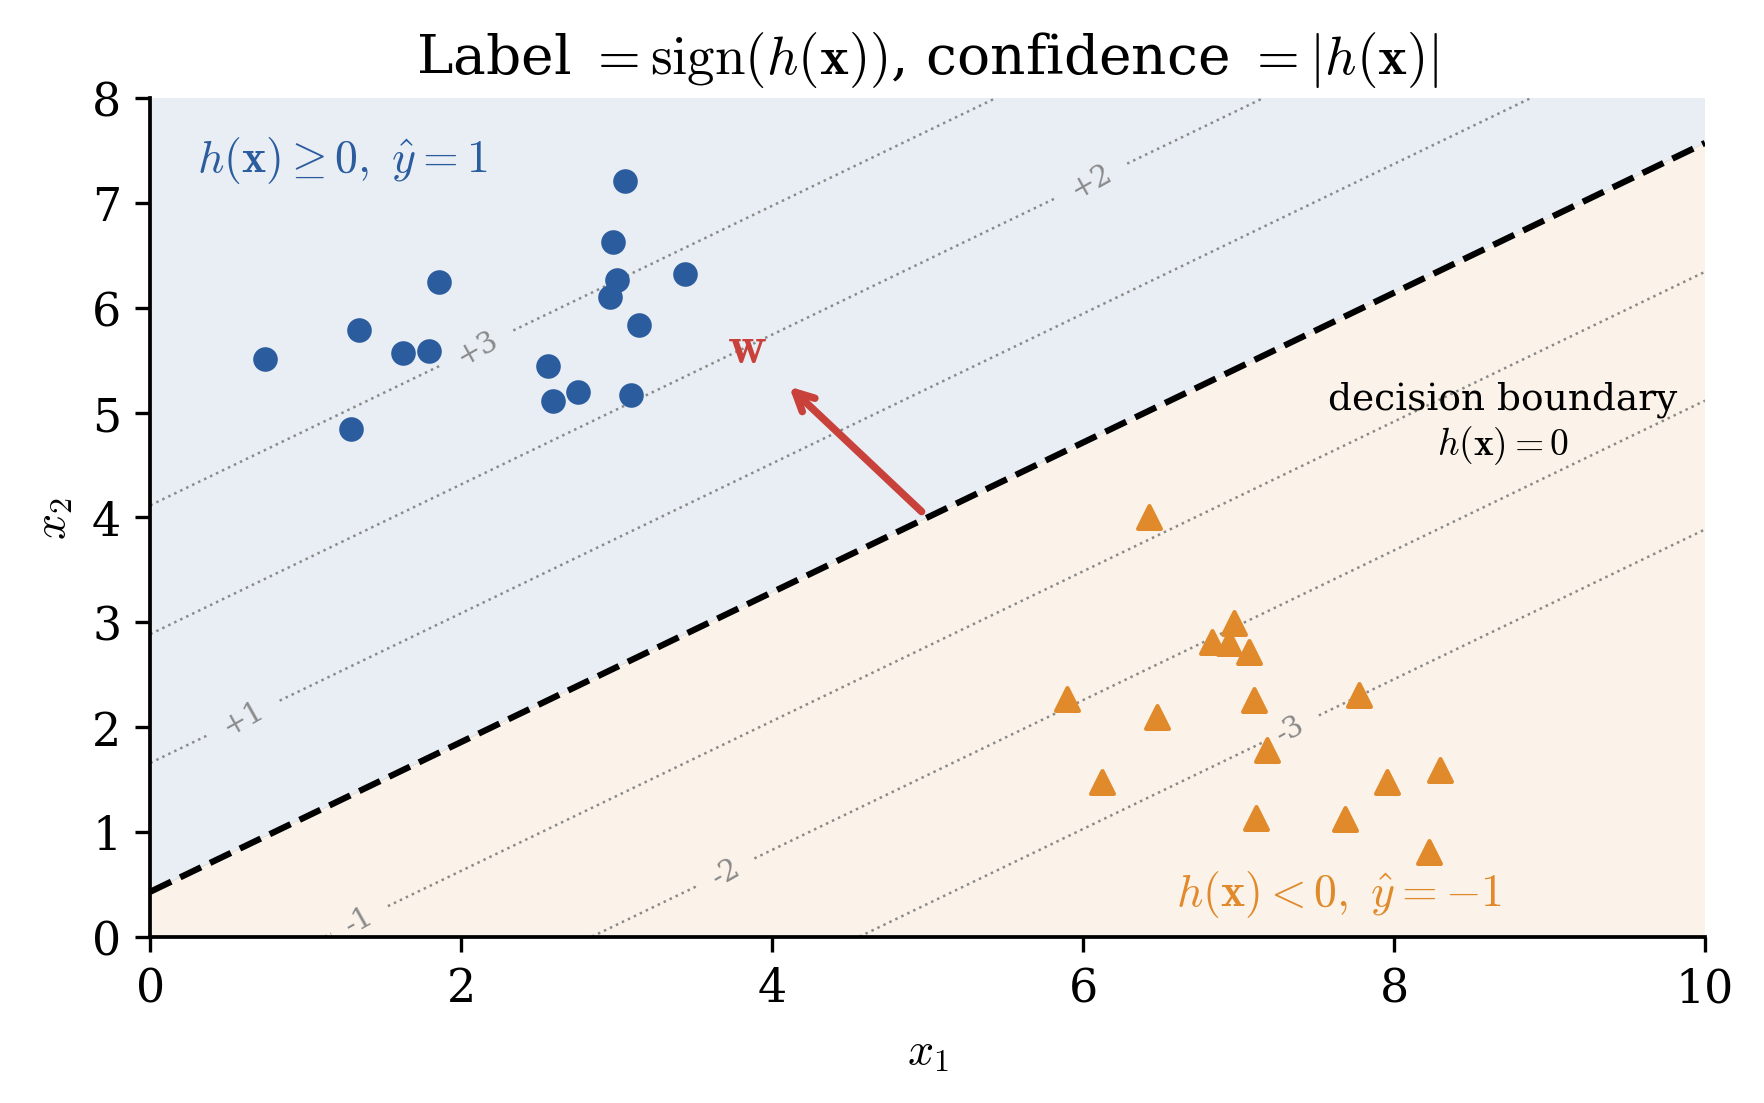
\includegraphics[width=0.7\textwidth]{images/chapter_6/sec_erm_classification.png}
    \caption{Linear classifier: label prediction and confidence}
\end{figure}

\subsection{Logistic Regression}
\textbf{Logistic Regression} is a binary classification method, and it is a clear example of the ERM recipe. It uses the same \textbf{data} (numeric features) and the same \textbf{model} (linear maps) as linear regression; the only thing that changes is the \textbf{loss}, which is the \textbf{logistic loss}:

\[
L\big((\mathbf{x},y),h\big) := \log\big(1 + \exp(-y h(\mathbf{x}))\big).
\]
The loss only depends on the product $y\,h(\mathbf{x})$. This product is positive when the predicted sign matches the true label (correct prediction) and negative otherwise. As a result:
\begin{itemize}
    \item correct and confident prediction ($y\,h(\mathbf{x})$ large and positive): the loss is close to zero;
    \item wrong prediction ($y\,h(\mathbf{x})$ negative): the loss grows, and it grows more the more confident the mistake is.
\end{itemize}

\begin{figure}[h]
    \centering
    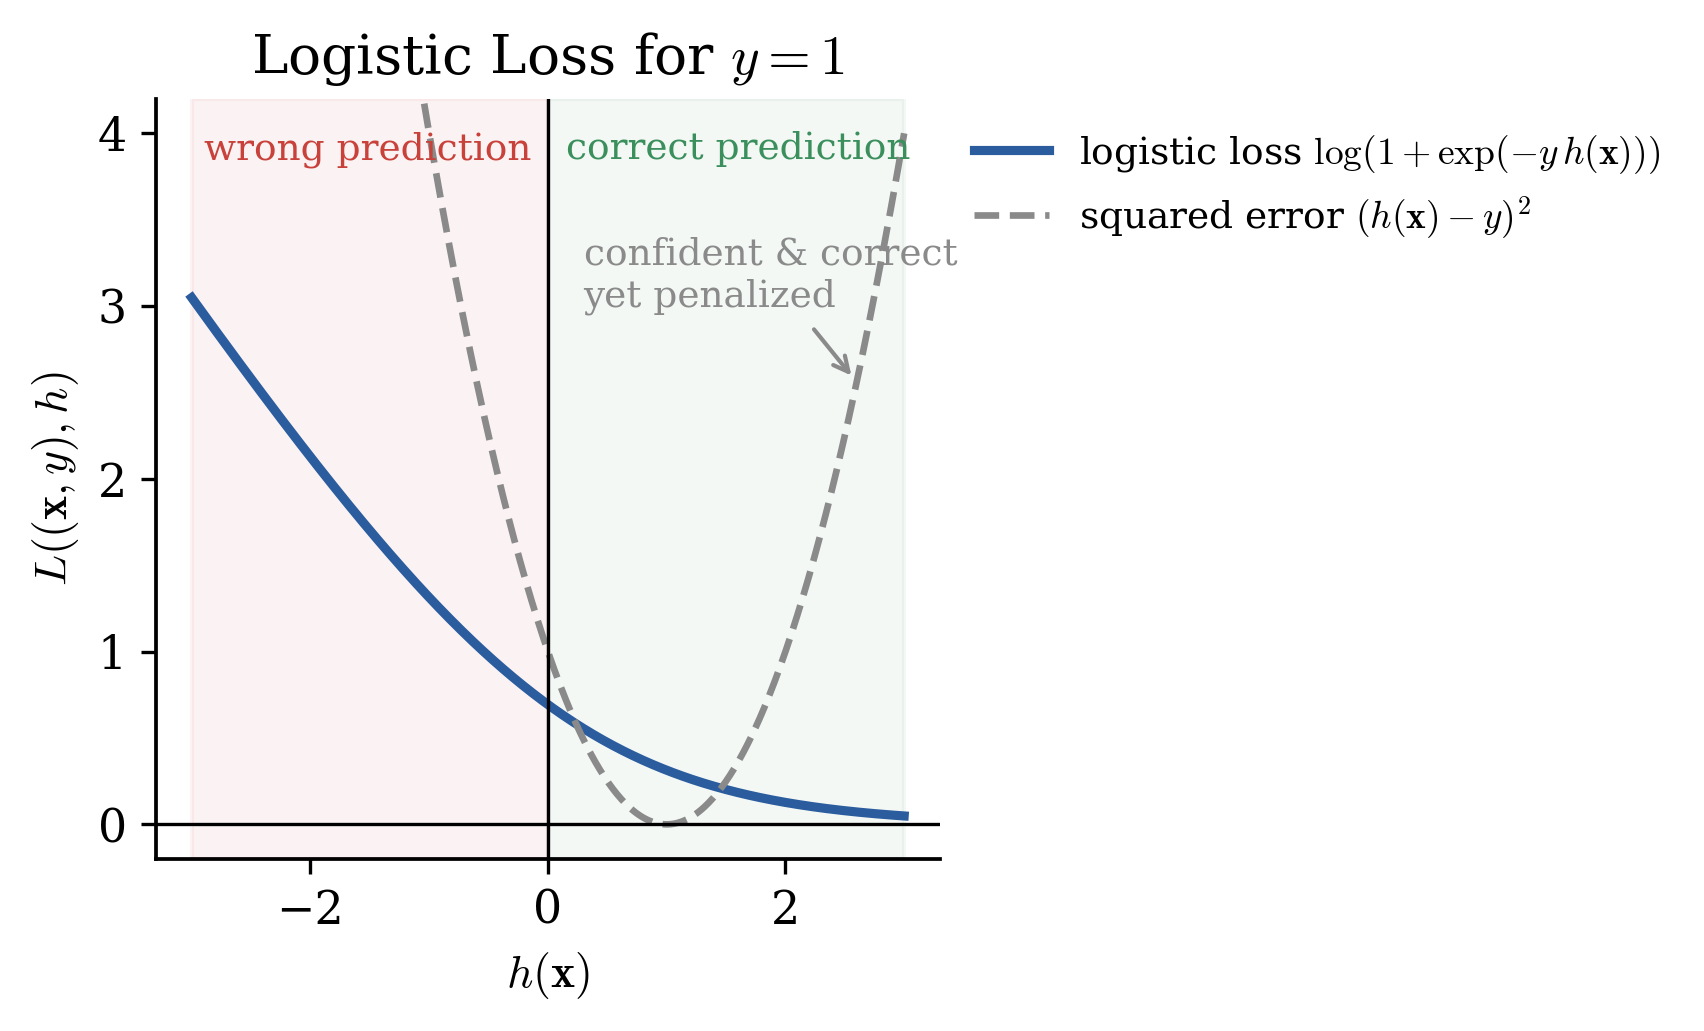
\includegraphics[width=0.85\textwidth]{images/chapter_6/sub_logistic_regression.png}
    \caption{Logistic Loss vs Squared Error Loss in classification}
\end{figure}

The logistic loss is \textbf{convex} and \textbf{differentiable}, so it is easy to minimize. The squared error loss, instead, is not suitable for classification. For example, if $y = 1$ and $h(\mathbf{x}) = 5$, the prediction is correct and very confident, yet the squared error is $(1-5)^2 = 16$. It \textbf{punishes the model for being confident and right}.

The \textbf{decision boundary}, i.e. the set of points where the classifier switches from one class to the other, is given by $h(\mathbf{x}) = 0$. Since $h$ is linear, this boundary is a straight line for two features (and a hyperplane in general).

\subsection{Loss Functions in Classification}
Besides the logistic loss, two other losses are common in classification:

\begin{itemize}
    \item \textbf{0/1 Loss}: it is $0$ if the prediction is correct and $1$ otherwise, so the empirical risk is simply the fraction of misclassified points. It measures exactly what we care about, but it ignores confidence and it is flat almost everywhere: it is \textbf{non-convex} and \textbf{non-differentiable}, and its gradient gives no direction to follow. For this reason it is used to \emph{evaluate} a classifier, not to train it.
    \item \textbf{Hinge Loss}: defined as $\max\big(0,\, 1 - y\,h(\mathbf{x})\big)$. It is zero when the prediction is correct with enough confidence ($y\,h(\mathbf{x}) \geq 1$) and grows linearly otherwise, so it also penalizes correct predictions that are not confident enough. It is \textbf{convex} but \textbf{not differentiable} at $y\,h(\mathbf{x}) = 1$. It is the loss used by Support Vector Machines.
\end{itemize}

\begin{figure}[h]
    \centering
    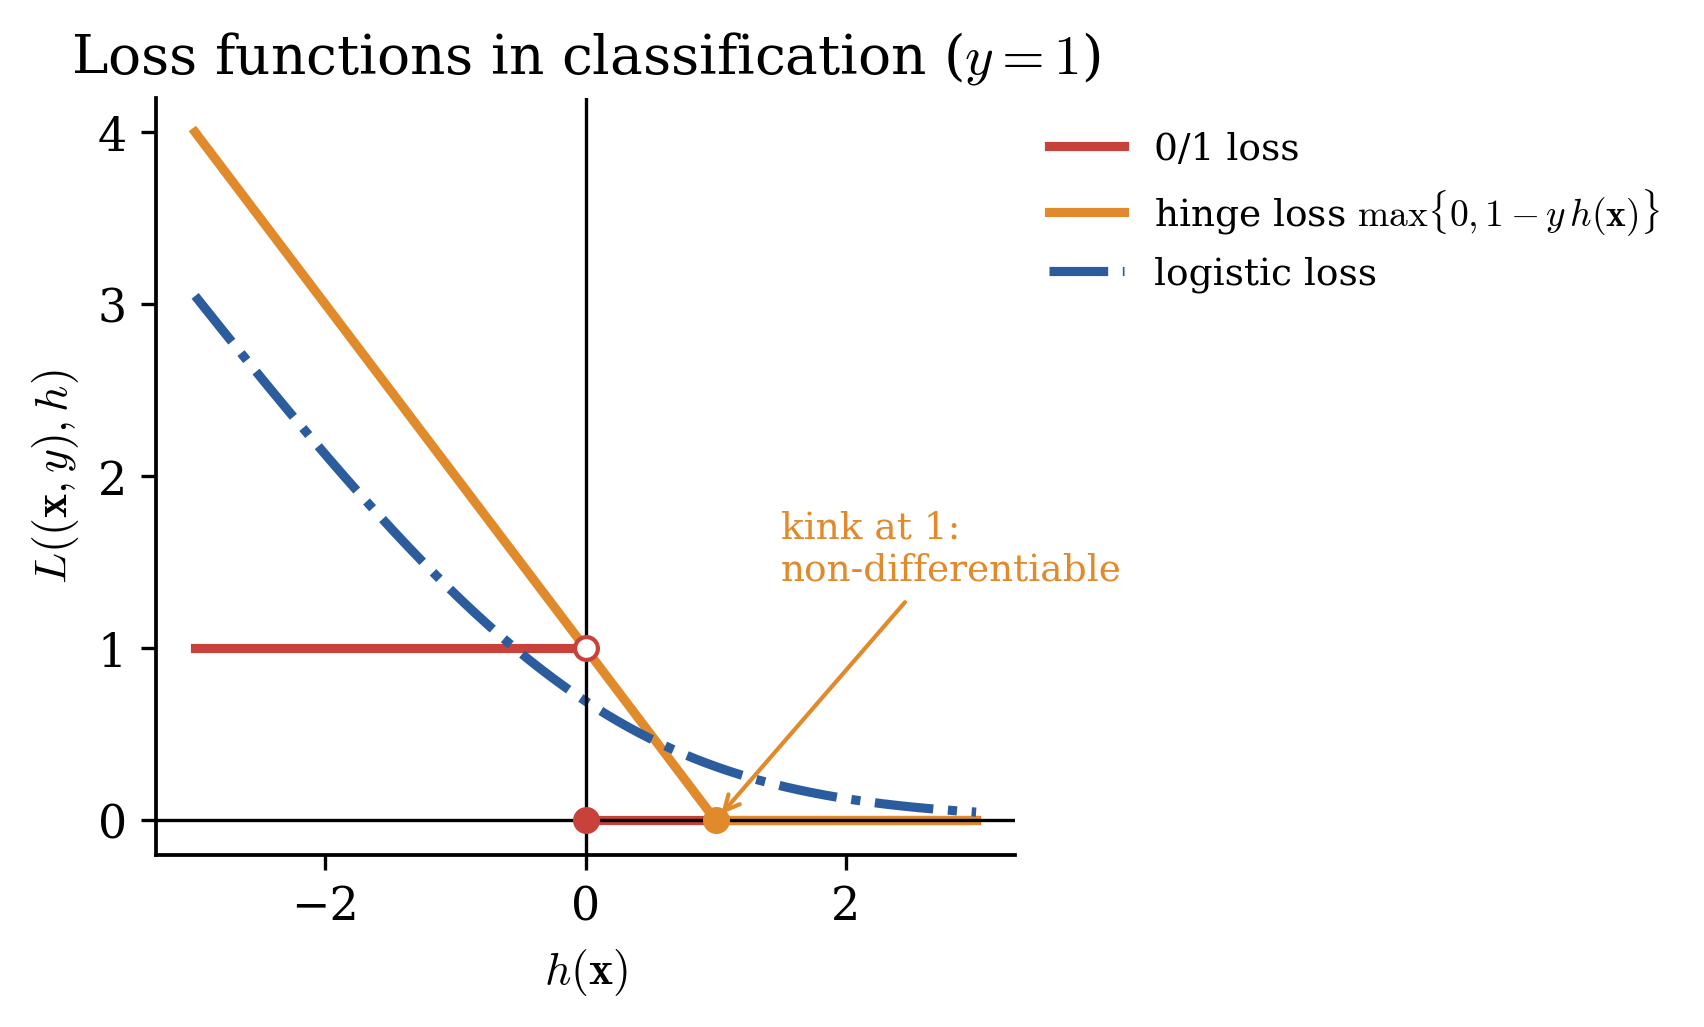
\includegraphics[width=0.6\textwidth]{images/chapter_6/sub_losses_classification.png}
    \caption{Loss functions in classification}
\end{figure}

\begin{center}
    \begin{tabular}{l|c|c|c}
        & \textbf{Uses confidence} & \textbf{Convex} & \textbf{Differentiable} \\ \hline
        0/1 Loss      & no  & no  & no  \\
        Hinge Loss    & yes & yes & no  \\
        Logistic Loss & yes & yes & yes \\
    \end{tabular}
\end{center}


\section{Summary}
\begin{figure}[h]
    \centering
    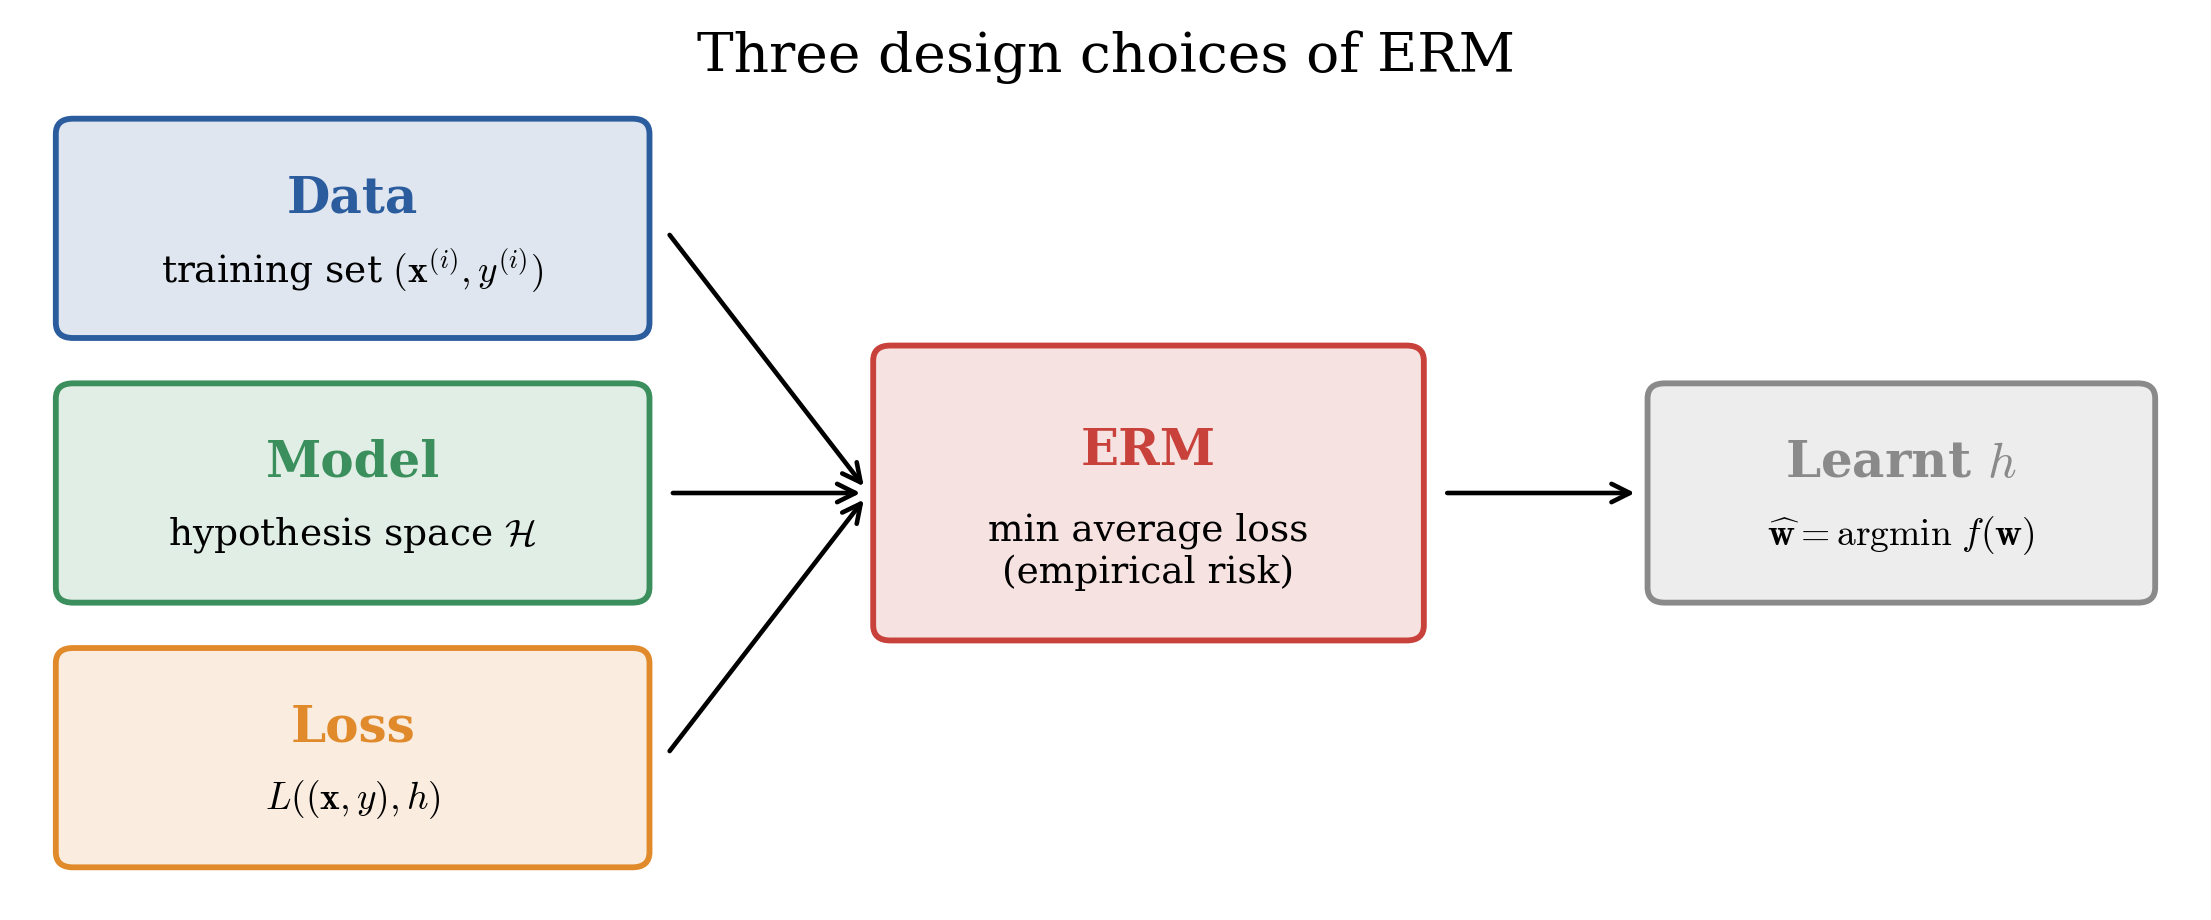
\includegraphics[width=0.5\textwidth]{images/chapter_6/sec_summary.png}
    \caption{Three design choices of ERM}
\end{figure}

\begin{itemize}
    \item The expected risk cannot be computed, so it is approximated by the \textbf{empirical risk}, the average loss on the training data.
    \item \textbf{ERM} learns the hypothesis with the smallest empirical risk. It can fail when the empirical risk is far from the expected risk.
    \item ERM is a general recipe based on \textbf{three design choices}: data, model and loss. Many ML methods are instances of ERM.
    \item Linear regression, polynomial regression and logistic regression are examples of ERM that differ only in some of these choices.
    \item In regression the loss measures a \textbf{distance} between numbers; in classification it is built from the \textbf{confidence} of the prediction.
    \item Convex and differentiable losses are preferred, since they are easier to minimize.
\end{itemize}





\section{A prova di coglione}

\subsection*{Il problema di fondo: non conosciamo la realtà}
Quello che vorremmo davvero è un'ipotesi $h$ che sbagli il meno possibile su \emph{qualsiasi} dato futuro, cioè che minimizzi il \textbf{rischio atteso}. Ma per calcolarlo servirebbe la distribuzione $p(x,y)$ da cui nascono i dati, e questa non la conosciamo mai. L'unica cosa che abbiamo è un campione: il training set.

L'idea centrale del capitolo è quindi una sostituzione: \textbf{al posto del rischio atteso usiamo la media delle loss sul training set}, il \textbf{rischio empirico}. Se i dati sono i.i.d. e abbastanza numerosi, la media sul campione è una buona stima della media sulla realtà. L'ERM consiste nello scegliere l'ipotesi che rende minima questa stima.

\begin{center}
    \fbox{\parbox{0.85\textwidth}{\centering
    \textbf{ERM è una scommessa:} che ciò che funziona bene sui dati di training funzioni bene anche sui dati che non abbiamo visto. Quando il rischio empirico si allontana da quello reale (pochi dati, dati non rappresentativi, modello troppo flessibile), la scommessa si perde.}}
\end{center}

\subsection*{ERM come ricetta: tre ingredienti}
L'ERM non è un singolo algoritmo ma uno \textbf{schema generale}. Per ottenere un metodo concreto bisogna fare tre scelte:
\begin{itemize}
    \item \textbf{Dati}: come rappresentiamo un punto (feature) e cosa vogliamo prevedere (label).
    \item \textbf{Modello}: lo spazio di ipotesi $\mathcal{H}$ tra cui cerchiamo, ad esempio tutte le funzioni lineari.
    \item \textbf{Loss}: come misuriamo quanto è grave un errore.
\end{itemize}

Cambiando anche uno solo degli ingredienti si ottiene un metodo diverso, ed è per questo che tanti metodi di ML sono in realtà casi particolari di ERM:

\begin{center}
    \begin{tabular}{l|l|l|l}
        & \textbf{Label} & \textbf{Modello} & \textbf{Loss} \\ \hline
        Linear Regression & numerica & mappe lineari & squared error \\
        Polynomial Regression & numerica & polinomi di grado $n$ & squared error \\
        Logistic Regression & binaria ($\pm 1$) & mappe lineari & logistic loss \\
    \end{tabular}
\end{center}

Notare che la Polynomial Regression non è un metodo nuovo: è la stessa regressione lineare applicata a feature trasformate ($x, x^2, \dots$). Si allarga il modello senza cambiare la ricetta.

Quando il modello è parametrizzato, cercare la migliore ipotesi equivale a cercare il miglior vettore di pesi: l'apprendimento diventa un \textbf{problema di ottimizzazione}, $\widehat{\mathbf{w}} = \operatorname{argmin}_{\mathbf{w}} f(\mathbf{w})$. Da qui l'importanza di loss \textbf{convesse} (un solo minimo, nessuna trappola) e \textbf{differenziabili} (il gradiente indica sempre la direzione in cui scendere).

\subsection*{La loss è dove decidiamo cosa conta}
La scelta della loss non è un dettaglio tecnico: \textbf{definisce che cosa significa ``sbagliare''}.

Nella \textbf{regressione} l'errore è una distanza tra numeri, e le tre loss viste sono tre atteggiamenti diversi verso gli errori grandi:
\begin{itemize}
    \item la \textbf{squared error} li punisce in modo quadratico, quindi è comoda da ottimizzare ma si lascia trascinare dagli outlier;
    \item la \textbf{absolute error} li tratta in proporzione, quindi è robusta agli outlier ma ha un punto angoloso in cui il gradiente non è definito;
    \item la \textbf{Huber loss} è il compromesso: quadratica per errori piccoli, lineare per quelli grandi. Prende il meglio delle altre due.
\end{itemize}

Nella \textbf{classificazione} la prospettiva cambia. Il modello produce comunque un numero $h(\mathbf{x})$, ma lo leggiamo in due parti: il \textbf{segno} dice la classe, il \textbf{modulo} dice quanto il modello ne è sicuro. Il confine tra le classi è dove $h(\mathbf{x}) = 0$, che per un modello lineare è una retta (o un iperpiano).

Una buona loss di classificazione deve quindi \textbf{premiare la sicurezza quando è giusta e punirla quando è sbagliata}. È esattamente qui che la squared error fallisce: penalizza un $h(\mathbf{x})$ molto grande anche quando la previsione è corretta, cioè punisce il modello per essere sicuro e nel giusto. La \textbf{logistic loss} invece decresce man mano che la previsione corretta diventa più sicura, ed è convessa e differenziabile. La \textbf{0/1 loss} conta semplicemente gli errori, ed è ciò che in fondo vogliamo misurare, ma è inutilizzabile come obiettivo da ottimizzare perché non è né convessa né differenziabile. La \textbf{hinge loss} è convessa ma ha un punto angoloso.

\subsection*{Il messaggio da portare a casa}
\begin{center}
    \fbox{\parbox{0.85\textwidth}{\centering
    Imparare significa \textbf{minimizzare l'errore medio sui dati che abbiamo}, sperando che rifletta l'errore sui dati che non abbiamo. Ogni metodo di ML nasce da tre scelte (dati, modello, loss), e la loss è quella che più di tutte decide sia \emph{cosa} il modello impara sia \emph{quanto facilmente} riusciamo a fargliela imparare.}}
\end{center}

